\documentclass[18pt,oneside,a4paper, titlepage]{article}

\usepackage[hidelinks]{hyperref}
\usepackage[pdftex]{graphicx}

\begin{document}
\begin{figure}[t]
	\centering
	
\includegraphics[scale=0.35]{logo-polimi.png}
\end{figure}
\title{\textbf{myTaxiService}\\\textbf{R}equirement \textbf{A}nalysis and \textbf{S}pecification \textbf{D}ocument\\ A.Y. 2015/2016\\
	Politecnico di Milano\\ Version 1.1}	
\author{Cattaneo Michela Gaia, matr. 791685\\Barlocco Mattia, matr. 792735 }
\date{November 6, 2015}
\maketitle

\newpage
\tableofcontents

\newpage
\section{Introduction}
	
	\subsection{Purpose}
		This document represents the Requirement Analysis and Specification Document (RASD). The aim of this document is to describe the system in terms of functional and non-functional requirements, modeling the system according to the real needs of the customer and showing the constraints and the limit of the software. This document serves as a contractual basis between the customer and the developer.
	
	\subsection{Actual system}
		The government of a large city has commissioned a system that is able to manage and optimize the taxi service.
	
	\subsection{Scope}
		The system aims at simplifying the access of the passengers and guaranteeing a fair management of taxi queues.
		In order to manage the queue optimization, the city is divided in zones, each one associated to a taxi queue, and the system computes the taxi distribution basing on their GPSs information.	\\	
		The system allows the user of the application to request a taxi in an area of the city, even without logging in, guaranteeing a fast way to access the service. As soon as a taxi driver takes the request, the application notifies the user of the ID of the incoming taxi and the waiting time. The user can also register, by filling in a form, and exploit additional functionalities such as choose the payment method he prefers or make reservations: he only needs to indicate the origin and destination of the ride and the exact time. \\
		On the other hand, the taxi driver always has to notify his availability and let the system know if he is going to take a certain request by a passenger. If the driver is not able to confirm, the system will forward the request to the second in the queue and will move this taxi driver in the last position of the queue.
	
	\subsection{Actors}
		The actors participating in the system are:
	\begin{itemize}
		\item Visitor: a person who can see the home page of the application, he can register, look up for information about the system and request a taxi, after providing e-mail address and phone number. 
		\item Passenger: a regular registered user who wants to use the application in order to request a taxi in a specific area or make a reservation for a given time.
		\item Taxi Driver: a registered user who logged in with a specific ID, provided by the system. This area is reserved to taxi drivers who needs to use the application in order to inform the system of their availability or about what request they are going to take care of.
	\end{itemize}
	
	\subsection{Goals}
	A user should be able to:
	\begin{itemize}
		\item Request a taxi.
		\item Check the waiting time.
		\item Visualize the information about the system.
		\item Sign up into the system.
	\end{itemize}
	A passenger should be able to:
	\begin{itemize}
		\item Log into the system.
		\item Reserve a taxi.
		\item Choose the payment method.
	\end{itemize}
	The taxi driver should be logged in with a specific ID and should be able to:
	\begin{itemize}
		\item Log into the system.
		\item Change his state from available to unavailable and vice versa.
		\item Visualize the queue of his area.
		\item Accept or decline the request that the system forwards to him.
		\item Visualize the position of the user he needs to reach.
	\end{itemize}

	\subsection{Domain properties}
	We suppose that the following properties hold in the analyzed domain.
	\begin{itemize}
		\item We assume that there are not previous implementations managing this service.
		\item The visitor is expected to be where he made the request to the system when the taxi driver arrives.
		\item The passenger is expected to be where and when he made the request to the system when the taxi driver arrives.
		\item The passenger is not supposed to cancel the reservation less than 2 hours earlier he has submitted it.
		\item A taxi driver always inform the system that he is available only when he actually is.
		\item A taxi driver, who notifies that he is going to take a certain request, always carries it out.
		\item At least one taxi driver in a queue accept the incoming request within few minutes.
		\item When a taxi driver finishes a ride, he instantly changes his state from unavailable to available.
		\item If a user requests a service from the system, it will be within the borders of the city.
		
	\end{itemize}


\newpage
\section{Overall Description}
	\subsection{Product perspective}
	The product consists in a web application and a mobile app both based on the web. The web application is used only by the users, the mobile app instead is used also by taxi drivers.\\
	There is a server which manages all the requests of the users along with the answers and the availability of the taxi drivers, computing their area distribution. There are several clients (visitors, passengers or taxi drivers) interacting with the server by using a graphical user interface, but there is no implementation of interfaces for administration. In fact, the application is only user-based.
	
	\subsection{User characteristics}
	The user can be a person who wants to request a taxi or access the system in order to use additional functionalities, such as make a reservation or easily request a taxi without having to give his information every time he exploits the service.
	The mobile app is used also by the taxi drivers who needs to receive the requests of the customers and to interact with the system, answering to the calls and updating their availability and their GPS position .
	
	\subsection{Constraints}
		\subsubsection{Regulatory policies}
		The system must ensure the privacy of the users, without publishing their personal information.
		\subsubsection{Hardware limitations}
		The system requires the users to use a device provided with a GPS detector and an Internet connection.
		\subsubsection{Interfaces to other applications}
		The system interfaces with three applications:
		\begin{itemize}
			\item Google Maps in order to determine the position of the taxi drivers and the users.
			\item Facebook if a user wants to sign in with his Facebook account.
			\item Google+ if a user wants to sign in with his Google+ account.
		\end{itemize}
		\subsubsection{Parallel operations}
			The system supports parallel operations of different clients, who access the application and make requests or reservations of taxis.
		
		\subsubsection{Documents related}
			\begin{itemize}
				\item Requirements Analysis and Specification Document (RASD).
				\item Design Document (DD).
				\item User's Manual.
				\item Testing report.
			\end{itemize}
		
		\subsection{Assumptions}
			\begin{itemize}
				\item The user can only make one request at a time, which means that the system does not allow him to make requests until the ride is over.
				\item The system changes the state of a taxi driver from available to unavailable if he accept a request, but not vice versa.
				\item If the passenger makes a reservation less then two hours in advance the system will not accept it.
				\item The user has to turn on his GPS in order to make any request.
				\item The system is able to manage the taxi queues in a way that there is always a taxi driver available for the reservation within ten minutes before the ride.
				\item The system deducts the cost of the ride from the credit card of the passenger only when the ride is over, sending also the receipt of the payment to the e-mail address indicated in the passenger profile.
				\item If the first taxi of the queue does not take the request, the system will send the request to the second taxi of the queue and, at the same time the first taxi will be moved in the last position of the queue.
				\item The taxi driver has one minute to answer the request, if he does not make it in time, the system considers it as declined.
				\item The profile of the passengers and of the taxi drivers are private, no other users or taxi drivers can visualize it.
				\item  The system constantly updates the position of all drivers of all areas, assigning their position to the correct queue of the area.
				\item When a user registers, the system does not instantly confirm the creation of a new passenger profile, but a confirmation e-mail is sent to the e-mail address provided by the user.
				\item When a passenger makes a reservation, the system retains it, then it forwards it to the first taxi driver in the queue of the designated area, ten minutes earlier the specified time.
				\item The taxi driver can not register in the application, but he will be added in the database, providing him his ID.
				\item There is always an available taxi driver in every area.
			\end{itemize}
			
		\subsection{Future possible implementations}
			The application is open to future implementations, which could be:
			\begin{itemize}
				\item Taxi sharing: this is an additional functionality that allows different passengers to share the taxi with other passengers. The system must be notified that the passenger wants to use the taxi sharing option and it will ask him to indicate the destination of this rides. When it is all settled, the system is able to check if there are other persons in the same area that wants to reach the same destination, informing the taxi driver and the passengers. This can be a convenient solution, as the cost of the ride would be equally shared among the passengers.
				\item Price transparency: this is an additional functionality that allows the passenger to calculate the price of the ride in advance, inserting its origin and destination.
				\item Meet the driver: this is an additional functionality that lets the passenger know which taxi driver has answered his request. The system will send the profile of the designated driver to the passenger, along with his name and data, so that the customer would be able to recognize him or even call or text him if necessary.
				\item Give us feedback: this is an additional functionality that allows the passenger to rate the driver after the ride and leave comments about it.
			\end{itemize}

\newpage
\section{Specific Requirements}
	\subsection{External interfaces requirements}
		\subsubsection{User interfaces}
			\begin{itemize}
				\item \textbf{Home page} This mockup represents the home page of the mobile app and of the web application, where a user can request a taxi or have access to the log in or registration page, or look up information about the service.
				\begin{figure}[h]
					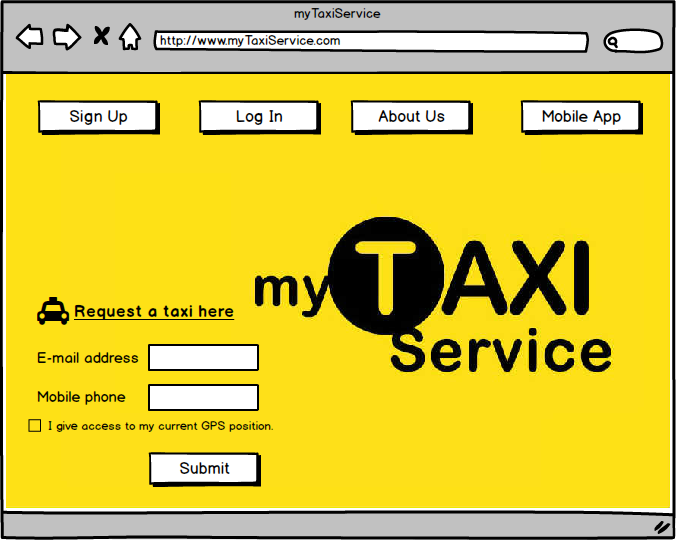
\includegraphics[scale=0.3]{Mockups/WebAppHomepage.png}%
					\qquad\qquad
					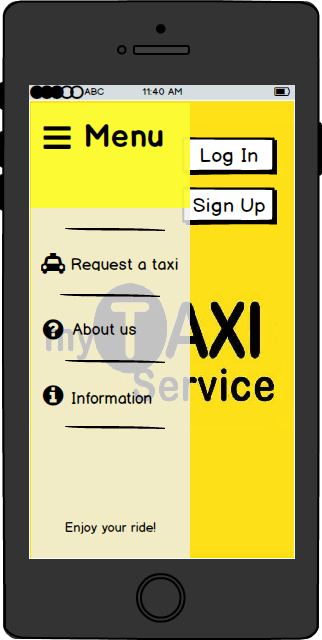
\includegraphics[scale=0.3]{Mockups/MobileAppHomepage.png}
				
				\end{figure}
				\\
				\item \textbf{Log in} This mockup represents the log in page of the mobile app and of the web application, where a user can log into the application filling in the form or accessing with the Facebook or Google+ account. The taxi drivers can use only the mobile application.
				\begin{figure}[h]
					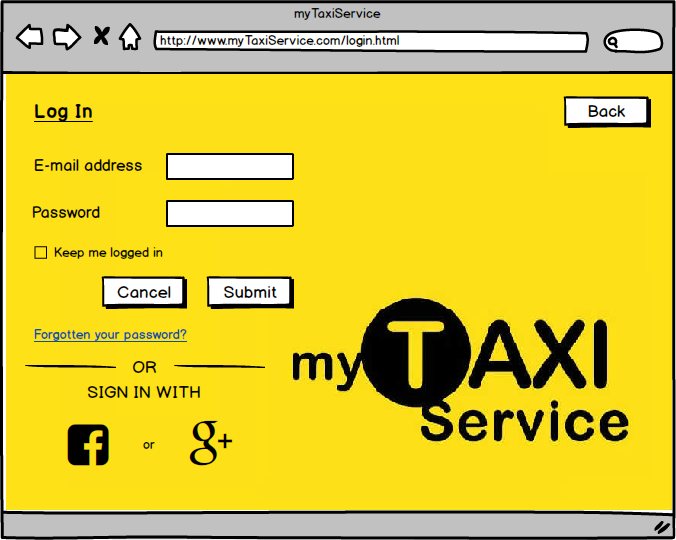
\includegraphics[scale=0.3]{Mockups/WebAppLogin.png}%
					\qquad\qquad
					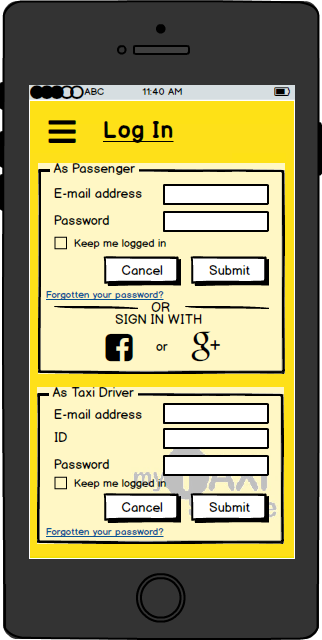
\includegraphics[scale=0.3]{Mockups/MobileAppLogin.png}
					
				\end{figure}
				\\
				\item \textbf{Registration} This mockup represents the sign up page of the mobile app and of the web application, where a user can register, filling in the form with his personal data.\\
				\begin{figure}[h]
					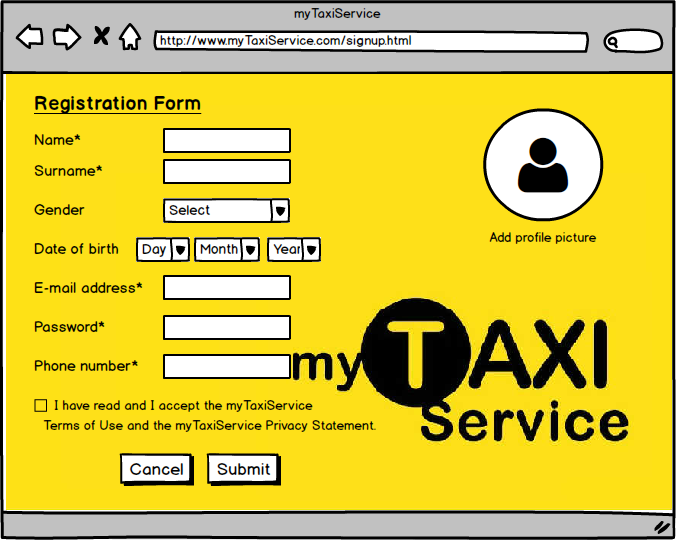
\includegraphics[scale=0.3]{Mockups/WebAppRegistration.png}%
					\qquad\qquad
					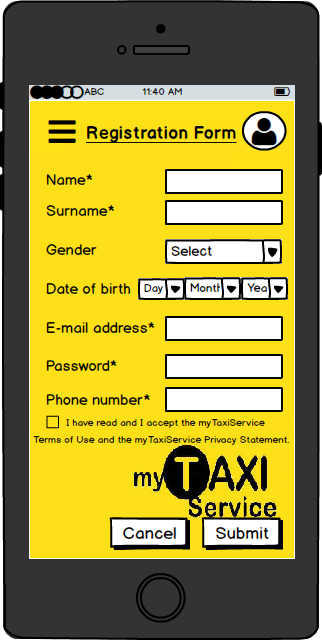
\includegraphics[scale=0.3]{Mockups/MobileAppRegistration.png}
				\end{figure}
				\\ 	\\
				\item \textbf{Passenger Area} This mockup represents the passenger area of the mobile app and of the web application, where a passenger can request or reserve a taxi or access to his profile.\\
				\begin{figure}[h]
					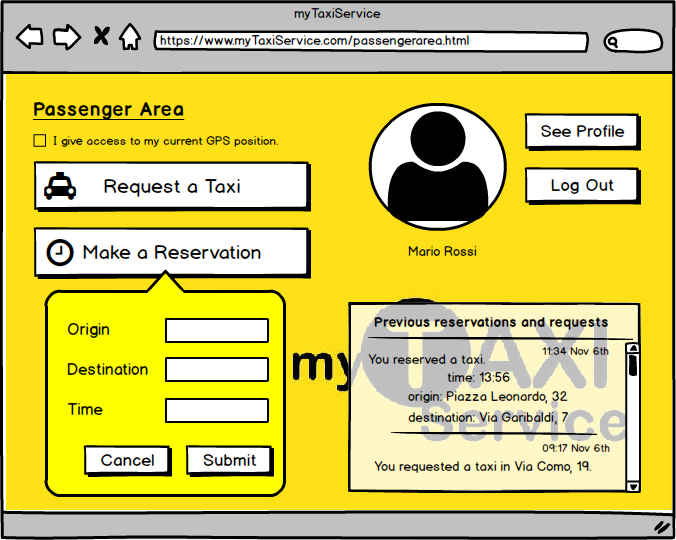
\includegraphics[scale=0.3]{Mockups/WebAppMakeAReservation.png}%
					\qquad\qquad
					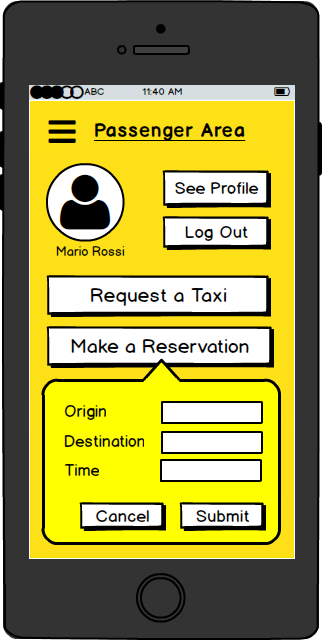
\includegraphics[scale=0.3]{Mockups/MobileAppMakeAReservation.png}
				\end{figure}
				\\ \\ \\
				\item \textbf{Payment Method} This mockup represents the passenger area of the mobile app and of the web application, where a passenger can choose the payment method of his request or reservation.\\
				\begin{figure}[h]
					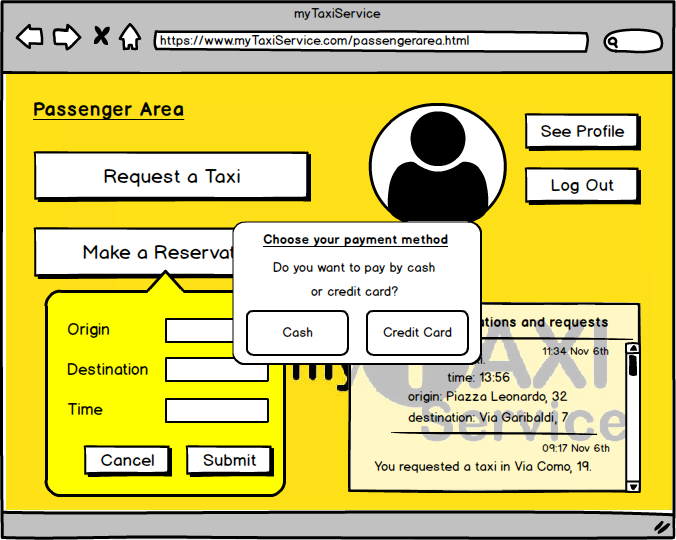
\includegraphics[scale=0.3]{Mockups/WebAppPaymentMethod.png}%
					\qquad\qquad
					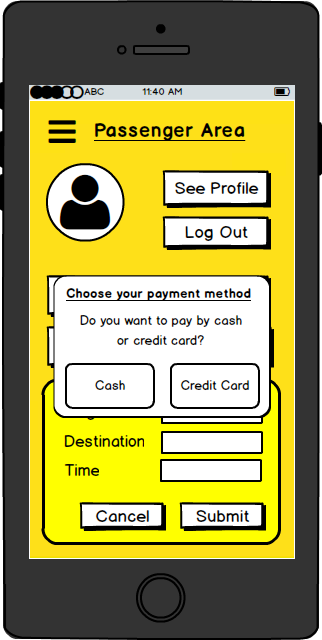
\includegraphics[scale=0.3]{Mockups/MobileAppPaymentMethod.png}
				\end{figure}
				\\ \\
				\item \textbf{Passenger Profile} This mockup represents the passenger profile mobile app and of the web application, where a passenger can see or modify his profile.\\
				\begin{figure}[h]
					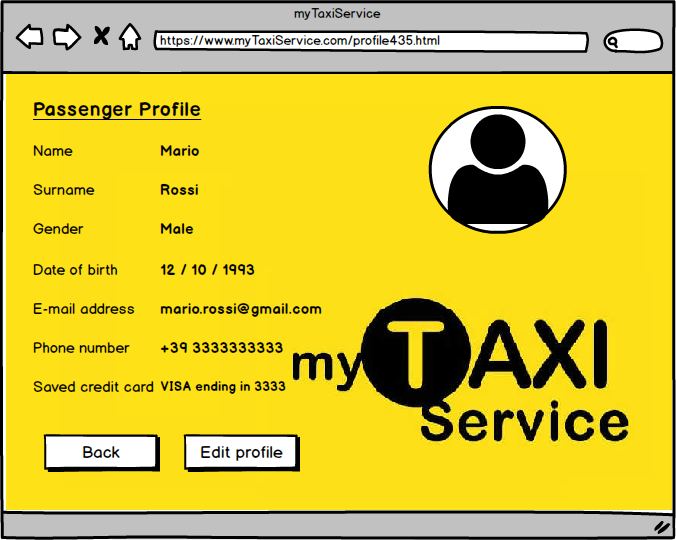
\includegraphics[scale=0.3]{Mockups/WebAppPassengerProfile.png}%
					\qquad\qquad
					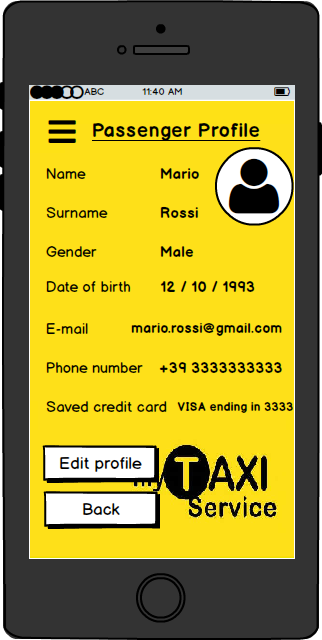
\includegraphics[scale=0.3]{Mockups/MobileAppPassengerProfile.png}
				\end{figure}
				\\ \\ \\ 
				\item \textbf{Credit Card Data} This mockup represents the passenger area of mobile app and of the web application, where a passenger can insert his credit card data.\\
				\begin{figure}[h]
					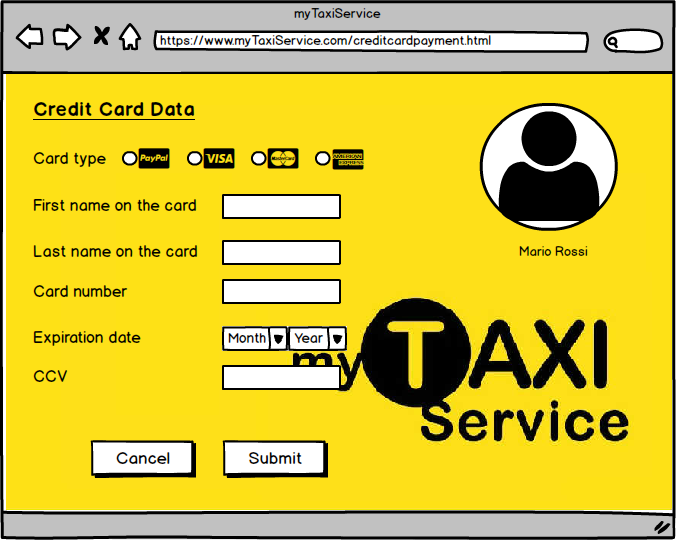
\includegraphics[scale=0.3]{Mockups/WebAppCreditCardData.png}%
					\qquad\qquad
					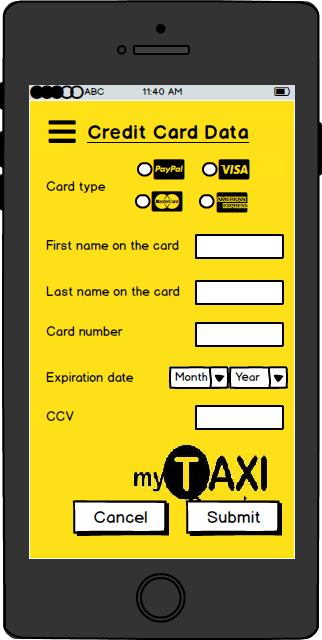
\includegraphics[scale=0.3]{Mockups/MobileAppCreditCardData.png}
				\end{figure}
				\\
				\item \textbf{Loading Screen} This mockup represents the passenger area of the mobile app and of the web application, where a passenger waits for his request to be taken in consideration and can cancel it.\\
				\begin{figure}[h]
					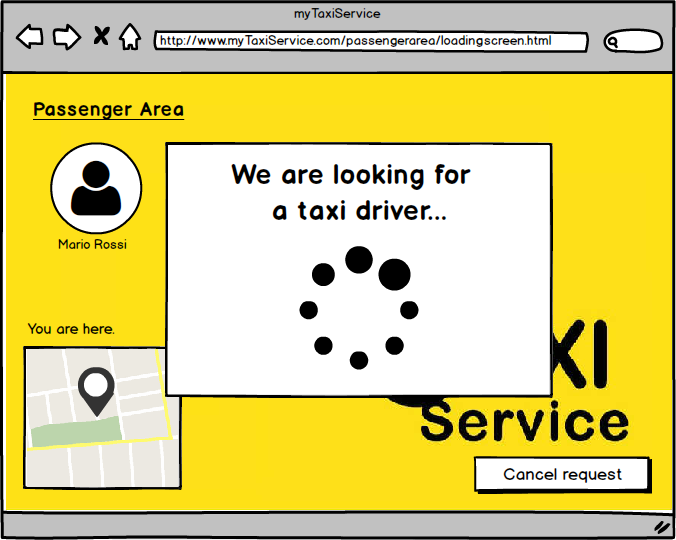
\includegraphics[scale=0.3]{Mockups/WebAppWaitForTaxi.png}%
					\qquad\qquad
					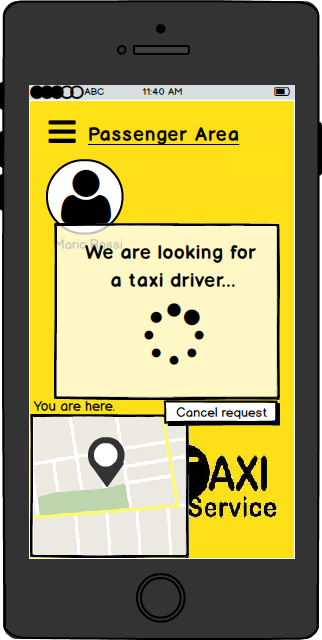
\includegraphics[scale=0.3]{Mockups/MobileAppWaitForTaxi.png}
				\end{figure}
				\\ \\ 
				\item \textbf{Waiting Time} This mockup represents the passenger area of the mobile app and of the web application, where a passenger see how much time he has to wait until the taxi arrival.\\
				\begin{figure}[h]
					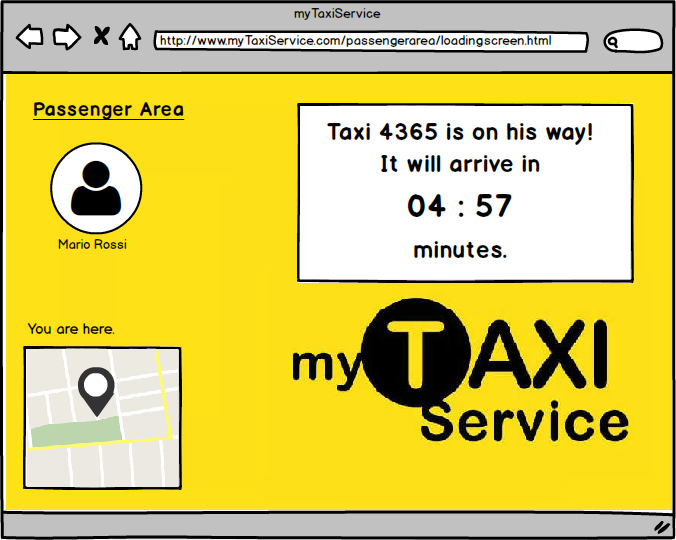
\includegraphics[scale=0.3]{Mockups/WebAppTaxiIsArriving.png}%
					\qquad\qquad
					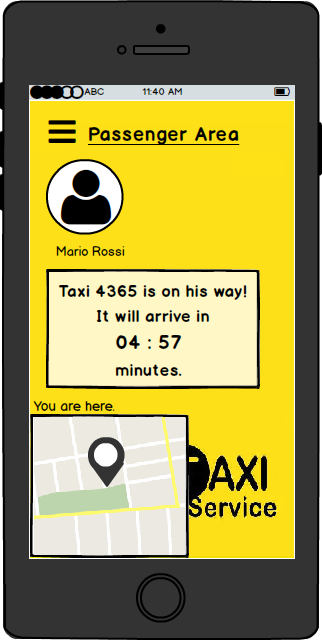
\includegraphics[scale=0.3]{Mockups/MobileAppTaxiIsArriving.png}
				\end{figure}
				\\ \\ \\
				\item \textbf{Taxi Driver Area} This mockup represents the taxi driver area of the mobile application, where a taxi driver can set his availability, see his position in the queue and access to his profile.\\
				\begin{figure}[h]
					\centering
					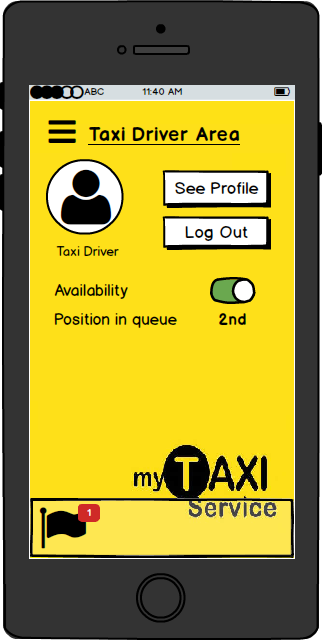
\includegraphics[scale=0.3]{Mockups/MobileAppTaxiDriverArea.png}
				\end{figure}
				\\
				\\ \\ 
				\item \textbf{Taxi Driver Notifications} This mockup represents the taxi driver area of the mobile application, where a taxi driver can see the notifications of the forwarded requests and accept or decline them.\\
				\begin{figure}[h]
					\centering
					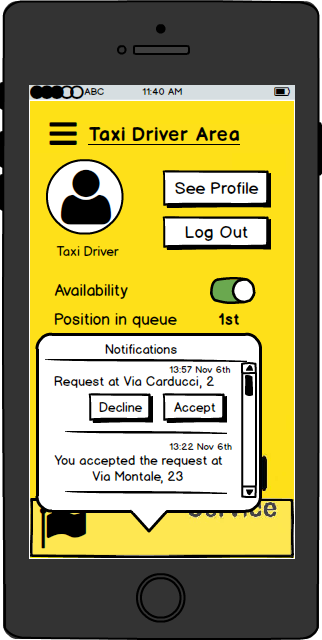
\includegraphics[scale=0.3]{Mockups/MobileAppTaxiDriverNotifications.png}
				\end{figure}
				\\
			\end{itemize}
\newpage
		\subsubsection{API interfaces}
			The system exploits the Google Map APIs in order to track the movements of the taxi drivers and to get the position of the users that request a service. It is necessary to be always aware of the taxi position in the areas and to make sure that the system is able to calculate the exact time the user has to wait until the taxi arrival. 
			Facebook and Google+ APIs are used to allow the users to log into the application without filling in any registration form or providing any further personal information.
			
		\subsubsection{Hardware interfaces}
			This project does not support any hardware interfaces.
		\subsubsection{Software interfaces}
			\begin{itemize}
				\item Database Management System (DBMS):
				\item[-] Name: MySQL.
				\item[-] Version: 5.6.21
				\item[-] Source: http://www.mysql.it/
				\item Java Virtual Machine (JVM).
				\item[-] Name: JEE
				\item[-] Version: 7
				\item[-] Source: http://www.oracle.com/technetwork/java/javaee/tech/index.html
				\item Application server:
				\item[-] Name: Glassfish.
				\item[-] Version: 4.1.
				\item[-] Source: https://glassfish.java.net/
				\item Operating System (OS).
				\item[-] Application must be able to run on any SO which supports JVM and
				DBMS specified before.
			\end{itemize}
		\subsubsection{Communication interfaces}
			\begin{center}
				\centering
			
				\begin{tabular}{|c| c| c|}
					\hline Protocol & Application & Port \\
					\hline		TCP & HTTPS & 443 \\
					\hline		TCP & HTTP & 80 \\
					\hline		TCP & DBMS & 3306(default)\\
					\hline
				\end{tabular}
			\end{center}
	\subsection{Functional requirements}
		\begin{itemize}
			\item \textbf{Registration of the visitor.}
				The system displays the registration form to the user, who needs to fill in the mandatory fields of the form and press the "Submit" button. The user should provide his name, surname, password, e-mail address and telephone number. He can choose whether let the system know about his gender and date of birth or not.
			
			\item \textbf{E-mail confirmation.}
				The system sends a confirmation e-mail is sent to the e-mail address provided by the user. The user can follow the link written in the e-mail and the system creates the new account.
				
			\item \textbf{Look up information about the system.}
				The system displays a screen where the user can read the data of the application, in particular the description of its functionalities, the contacts of the managers of the system and information about the investors.
				
			\item \textbf{Log in as a passenger.}
				The system provides an input form where the passenger can insert e-mail and password. The system checks if the account is already registered and if the password is correct, if not an error message is displayed. If this conditions hold, the passenger logs in successfully.
				
			\item \textbf{Log in as a taxi driver.}
				The system provides an input form in the mobile application where the taxi driver can insert e-mail, ID and password. The system checks if the account is correctly registered, if the ID matches the e-mail address and if the password is correct, if not an error message is displayed. If this conditions hold, the taxi driver logs in successfully.
				
			\item \textbf{Log in with social networks}
				The system allows the user to sign up with his Facebook or Google+ account without inserting e-mail, telephone number and the other information, if he has already inserted them on his profile.
				
			\item \textbf{Retrieve password.}
				The system provide a link to recover the password of the account. The user clicks on the link and receives a recover e-mail with a link that redirects to a page where he can set his new password.
				
			\item \textbf{Request a taxi.}
				The user can make taxi requests enabling the GPS of his device so that the system can determine his position and send the call to the first taxi driver of the queue of the designated area.
				The visitor can exploit this service in the home page of the application, inserting his e-mail and telephone number.
				The passenger can use this service in the passenger area, displayed after the log in, without inserting any further information.
				
			\item \textbf{Reserve a taxi.}
				The system provides a "Make a reservation" button in the passenger area. The passenger presses this button and an input form is displayed, where he should indicate the origin, destination and time of the ride.
				
				\newpage
			\item \textbf{Choose payment method.}
				The system, after the passenger submits a request or a reservation, displays a panel to him, where he can choose whether to use cash or credit card as payment method. If the passenger decides to pay by cash, the taxi driver will take care of the payment. Instead the passenger needs to add his credit card data only if this is the first time he chooses this payment method, in fact the system adds the credit card data to his profile after the insertion and does not ask anymore. 
				
			\item \textbf{View the profile.}
				The passenger or the taxi driver can see his profile by pressing the "See profile" button. The system displays a screen with his personal data already inserted and his profile picture.
				
			\item \textbf{Edit the profile.}
				 The passenger can edit his profile by pressing the "Edit profile" button and the system displays a screen where he can change his name, surname, e-mail address, password, phone number and profile picture. He can edit or add his gender, date of birth and credit card data. In case the passenger modifies his e-mail address, the system will send an e-mail confirmation.
				 
			\item \textbf{See waiting time.}
				The system displays to the user who has made a request the waiting time panel, from the time a taxi driver is found until he arrives. The user can see the panel to know how much time he has to wait till the taxi arrival.
				
			\item \textbf{Change availability.}
				The taxi driver can switch his state from available to unavailable and vice versa. The system does not consider him in the queue as long as his state is unavailable and, if he is available, the system shows him his queue positioning and keeps him in consideration for the requests of the users.
				
			\item \textbf{Notification of the requests.}
				The taxi driver can see the requests by a user as notifications in the notification panel. The system sends him a notification with the position of the user, the taxi driver can decide to accept the request or refuse it.
				
			\item \textbf{See position in the queue.}
				The system provides the taxi driver his position in the queue in his area, if his state is set to available, so that he is always able to know if there can be any incoming requests.
				
		\end{itemize}
\newpage
	\subsection{Non-functional requirements}
		\subsubsection{Performance requirements}
			The system is composed of a server side hosting the database, where all the data of the passenger and of the taxi driver are stored, and it handles all the HTTP request. There is not a great amount of data to manage: there are the profile information of the passengers, of the taxi drivers and the log of the activities; so the size of the database is not a constraint for the system.\\ In order to provide a suitable service, the system has to be reactive and able to answer to a high number of simultaneous requests.\\ There are no time constraints that depends on the system, the time to process a transaction is less then one second. The only time constraint would be the reply message of the taxi driver that depends on his reflexes.
		\subsubsection{Software system attributes} 
			\begin{enumerate}
				\item Reliability: the server must remain up twenty-four hours a day in order to guarantee a suitable service. The system allows the administrators to fix any problem without compromising the functionality of the system.
				\item Availability: in order to guarantee the continuous availability of the data, it has been arranged one backup system on a secondary database and the other on an external storage. 
				\item Security: privacy of the data exchanged between the server and the clients is guaranteed by a SSL encryption. The passwords and the sensitive data stored on the database are protected by MD5 encryption.
				\item Portability: the client side of the system is compatible with the major mobile platforms on the market (e.g. Android, iOS) and any device (e.g. PC with Windows, Apple, etc.) that supports a browser and a GPS system.
			\end{enumerate}
\newpage
\section{Scenarios Identifying}
	\subsection{Scenario 1: Registration and log in}
		Virginia is new to the city and is not used to use public transport, so she searches for the best taxi services via web. After a while, she decides to download the new application "myTaxiService", because it seems to offer the most interesting functionalities. Virginia registers in the application, without even filling the form, accessing with her Facebook account and adds her favorite photo with her boyfriend. Now she is able to log in, to make taxi reservations choosing the payment method she prefers and to request a taxi without having to insert her information every time she needs it.
		
	\subsection{Scenario 2: Password recovery}
		Charlie has registered in the application when he visited the city a few months ago, now he is back and needs to make a taxi reservation for the afternoon. But Charlie is really absent-minded and is not able to remember his password. He is very happy to see the "Forgotten your password?" link and he press it: this leads to another page where the system tells him that an e-mail for the recovery has been sent to his e-mail address. He checks his inbox and follows the link to set his new password. Now he can easily log in and make his reservation.
		
	\subsection{Scenario 3: Choose payment method}
		William often uses myTaxiService for the taxi requests, as it is a fast and reliable service. He is a very lazy person and does not want to register, as the application allows visitors to easily request a taxi, but he is very tired of paying by cash, so he finally make up his mind. He registers and adds his credit card data to his profile. William is happy to save his time and he can request or reserve a taxi without even worry about the money spent.
	
	\subsection{Scenario 4: Reserve a taxi}
		Pierre asks his friend next door, Marie, out for a date at the restaurant and then at the cinema. He really wants to make a good impression, but his car is at the mechanic. So Pierre decides to go anyway by bus, even tho it is not the most elegant solution, but when he will come back there will not be any public transport. He decides to register in the myTaxiService application and make a reservation for 00:30 pm, when the movie ends. The taxi is already there when they come out of the cinema and they are home in a few minutes, Pierre and Marie are very satisfied with the service and with the evening too.
		\newpage
	\subsection{Scenario 5: Taxi driver availability}
		Jonathan is used to take a coffee after his first ride of the day. Even if he is the first of the queue, he wants to maintain this habit, so he just switch his availability button to off. Now the system knows that he cannot be called for the requests and he can set his state available whenever he wants and see his position in the queue. Finally, when Jonathan takes a call, he knows that he does not have to bother about his availability because the system always sets his state unavailable in the exact time he takes the request of a passenger.
		
	\subsection{Scenario 6: Taxi drivers notification of the requests}
		Walter is the first of the queue, so he knows that he is going to take a request soon but he is on the phone with his mother and does not see the notification within the first minute, so the system forwards it to the second taxi driver of the queue. Now he is in the last position of the area and needs to be very careful when the positions change. Walter shifts fast to the first position again and he is now able to click on the "Accept" button before the time is over. He sees the position of the request and goes there with no trouble. At the end of the day he scrolls his notifications panel and he is very satisfied with his work today, as he has missed just one request.
\newpage
\section{UML Models}
	\subsection{Use Case diagram}
	This Use Case diagram gives an overview on the main actors of the system and their functionalities.
	\\
	\begin{figure}[h]
		\centering
		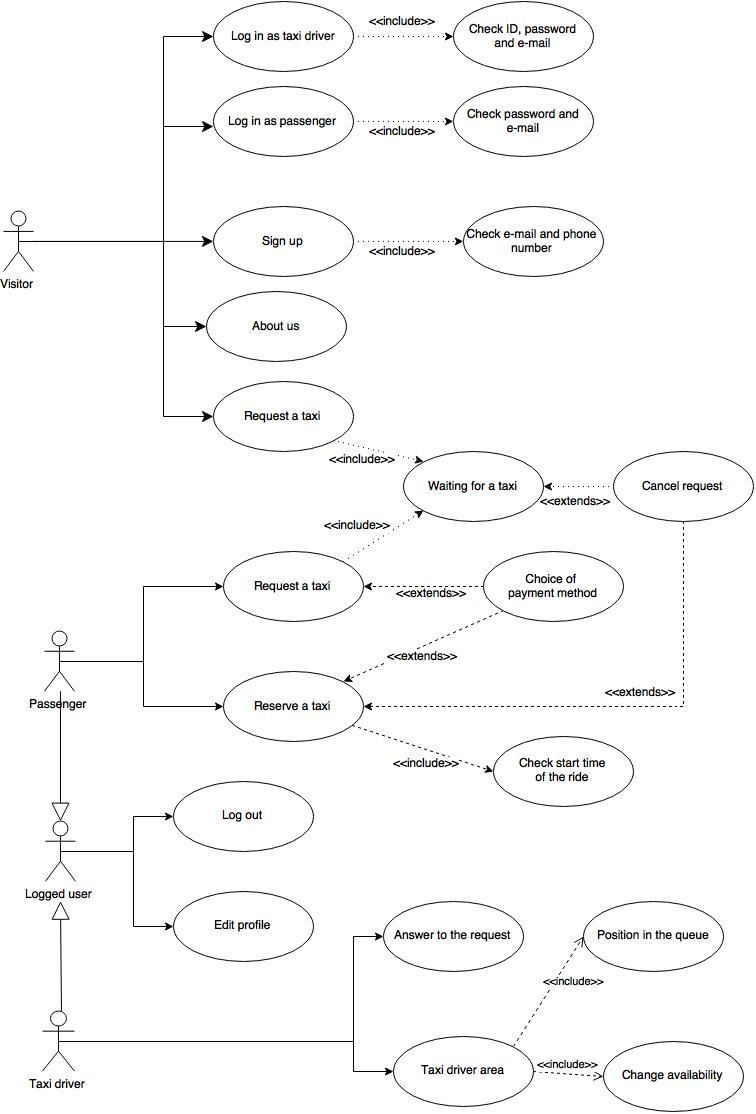
\includegraphics[scale=0.4]{Diagrams/UseCase2.jpg}
		
	\end{figure}
\newpage
	\subsection{Class diagram}
	This Class diagram describes a basic structure of the entities of the system and their relations.
	\\ \\ \\ 
	\begin{figure}[h]
		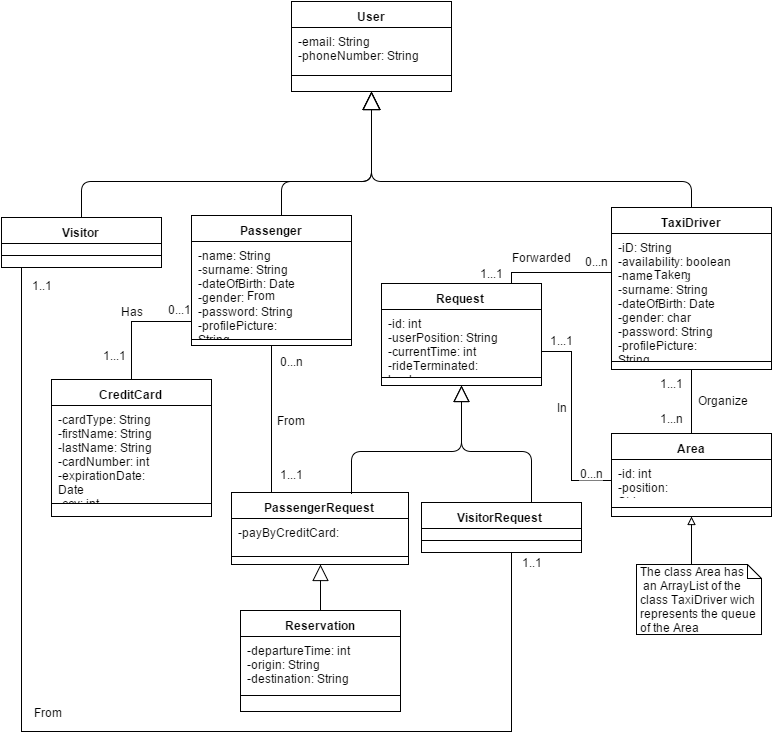
\includegraphics[scale=0.55]{Diagrams/classDiagram.png}
	\end{figure}
\newpage
	\subsection{Sequence diagram}
	\begin{itemize}
		\item User Registration
		\\ \\ \\
		\begin{center}
			\centering
			
			\begin{tabular}{| c| p{8cm}|}
				\hline \textbf{Actor} &  Visitor and passenger.\\
				\hline \textbf{Goal} & Sign up into the system.\\
				\hline \textbf{Input Condition} & The visitor is not already registered into the system. \\
				\hline \textbf{Event Flow} & 1.	The system shows the sign up page.\\
				& 2. The visitor completes the sign up form and submits.	\\
				\hline \textbf{Output Condition} & 1. The system checks the information  of th e visitor and allows him to log in\\
				& 2. The visitor becomes a passenger.\\
				\hline \textbf{Exception} & If any information is incorrect, the system notifies the visitor and asks him to redo it.\\
				\hline
			\end{tabular}
			\vspace{4cm}
			\begin{figure}[h]
				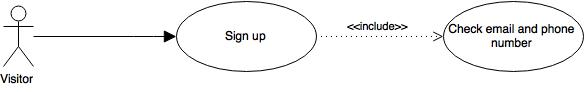
\includegraphics[scale=0.71]{Diagrams/UseCaseSignup.jpg}
			\end{figure}
		\end{center}
		
		\newpage
		
		\begin{figure}[h]
			\centering
			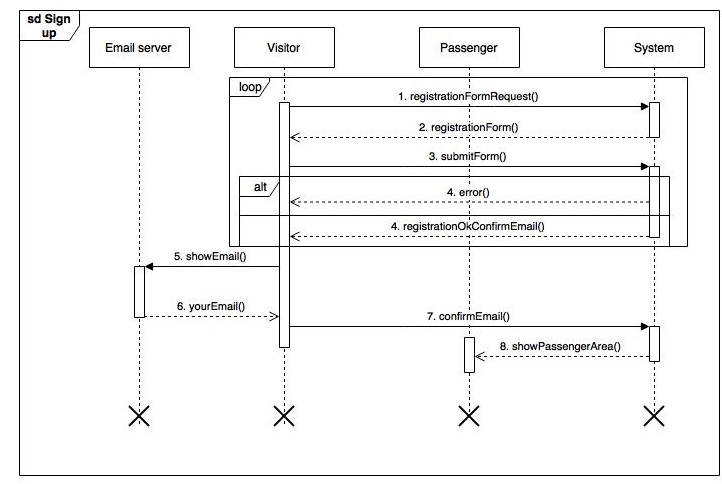
\includegraphics[scale=0.71]{Diagrams/SequenceSignup.jpg}
		\end{figure}
		\newpage
		\item User Log In
		\\ \\ \\
		\begin{center}
			\centering
			\begin{tabular}{|c|p{8cm}|}
				\hline \textbf{Actor} &  Visitor, taxi driver and passenger.\\
				\hline \textbf{Goal} &  Log into the system.\\
				\hline \textbf{Input Condition} & The visitor is already registered into the system as a taxi driver or a passenger.\\
				\hline \textbf{Event Flow} & 1. The system shows the login page.\\
				& 2. The visitor completes the login form.\\
				\hline \textbf{Output Condition} & 1. The system checks the credentials and shows the passenger or taxi driver area.\\
				& 2. The visitor becomes a passenger or a taxi driver if the credentials are correct.\\
				\hline \textbf{Exception} & If the credentials are incorrect the system notifies the visitor.\\
				\hline
			\end{tabular}
			\vspace{4cm}
			\begin{figure}[h]
				\centering
				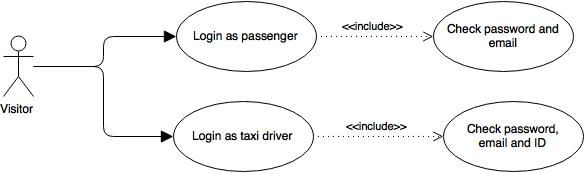
\includegraphics[scale=0.6]{Diagrams/UseCaseLogin.jpg}
			\end{figure}
		\end{center}
		
		\newpage
		 
		\begin{figure}[h]
			\centering
			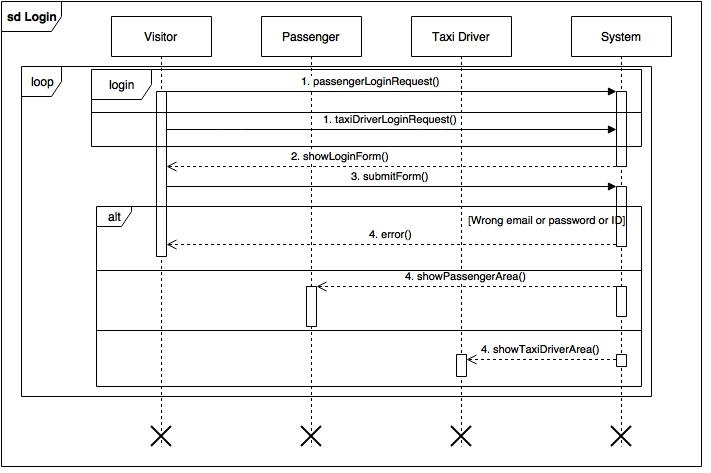
\includegraphics[scale=0.75]{Diagrams/SequenceLogin.jpg}
		\end{figure}
			\newpage
			\item Passenger Profile
			\\ \\ \\
			\begin{center}
				\centering
				\begin{tabular}{|c|p{8cm}|}
					\hline \textbf{Actor} &  Passenger.\\
					\hline \textbf{Goal} & Edit his profile information.\\
					\hline \textbf{Input Condition} & The passenger is already logged in.\\
					\hline \textbf{Event Flow} & 1.	The system shows the “Edit profile” page.\\
					& 2. The passenger modifies some information and submits the changes.\\
					\hline \textbf{Output Condition} & The system checks the changes and shows the passenger area.\\
					\hline \textbf{Exception} & If any information is incorrect, the system notifies the passenger and cancels the changes.\\
					\hline
				\end{tabular}
				\vspace{4cm}
				\begin{figure}[h]
					\centering
					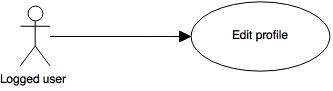
\includegraphics[scale=0.8]{Diagrams/UseCaseProfile.jpg}
				\end{figure}
			\end{center}
			
			\newpage
			
			\begin{figure}[h]
				\centering
				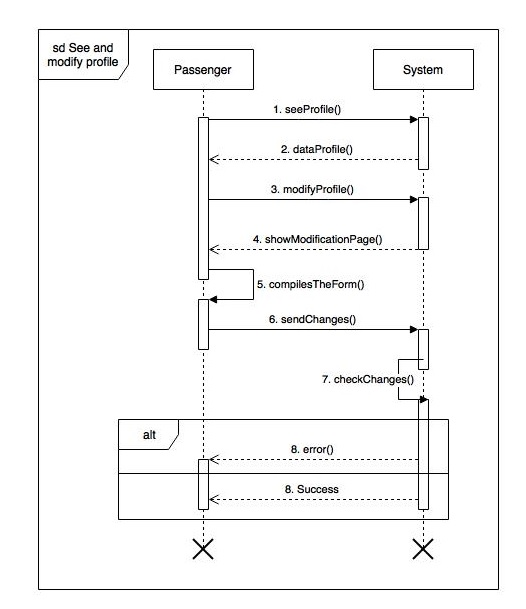
\includegraphics[scale=0.97]{Diagrams/SequenceProfile.jpg}
			\end{figure}
			\newpage
			\item Request By A User
			\\ \\ \\
			\begin{center}
				\centering
				\begin{tabular}{|c|p{8cm}|}
					\hline \textbf{Actor} & Taxi driver and passenger.\\
					\hline \textbf{Goal} & Request a taxi and answer to the request.\\
					\hline \textbf{Input Condition} & The passenger is already logged in and he has not made any request or reservation recently.\\
					\hline \textbf{Event Flow} & 1.	The passenger presses the request button.\\
					& 2. The passenger waits for the system to look for an available taxi driver.\\
					& 3. The taxi driver answers to the request.\\
					& 4. The system sends a confirmation to the passenger if a taxi driver has accepted the request. \\
					\hline \textbf{Output Condition} & When the system finds a taxi driver, it notifies the passenger.\\
					\hline \textbf{Exception} & If a taxi driver declines the request, the system continues the research.\\
					\hline
				\end{tabular}
				\vspace{1cm}
				\begin{figure}[h]
					\centering
					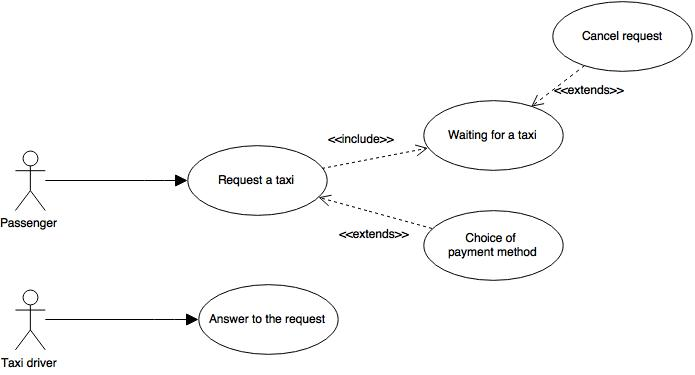
\includegraphics[scale=0.6]{Diagrams/UseCaseRequest.jpg}
				\end{figure}
			\end{center}
			
			\newpage
			
			\begin{figure}[h]
				\centering
				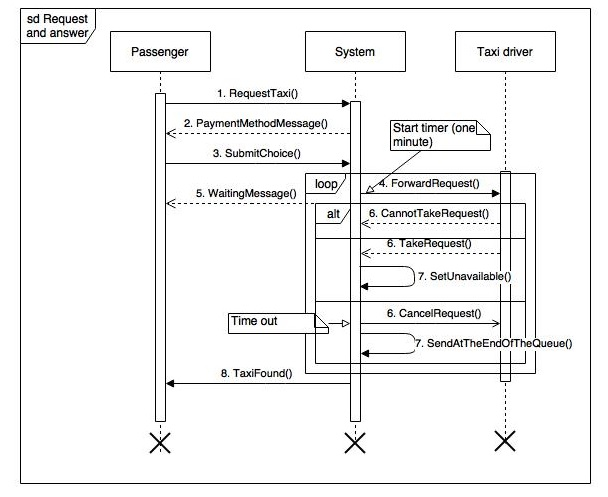
\includegraphics[scale=0.9]{Diagrams/SequenceRequest.jpg}
			\end{figure}
				\newpage
				\item Reservation By A Passenger
				\\ \\ \\
				\begin{center}
					\centering
					\begin{tabular}{|c|p{8cm}|}
						\hline \textbf{Actor} &  Taxi driver and passenger.\\
						\hline \textbf{Goal} & Reserve a taxi and answer to the request.\\
						\hline \textbf{Input Condition} & The passenger is already logged in and he has not made any request or reservation recently.\\
						\hline \textbf{Event Flow} & 1.	The passenger presses the “Make a reservation” button.\\
						& 2. The system displays to the passenger the reservation form.\\
						& 3. The passenger fills in the form and submits it.\\
						& 4. The system checks the current and the departure time.\\
						& 5. Ten minutes before the ride, the system looks for an available taxi driver. \\
						\hline \textbf{Output Condition} & When the system finds a taxi driver, it notifies it to the passenger.\\
						\hline \textbf{Exception} & If the departure time is wrong, the system does not allow the passenger to make the reservation.\\
						\hline
					\end{tabular}
					\vspace{1cm}
					\begin{figure}[h]
						\centering
						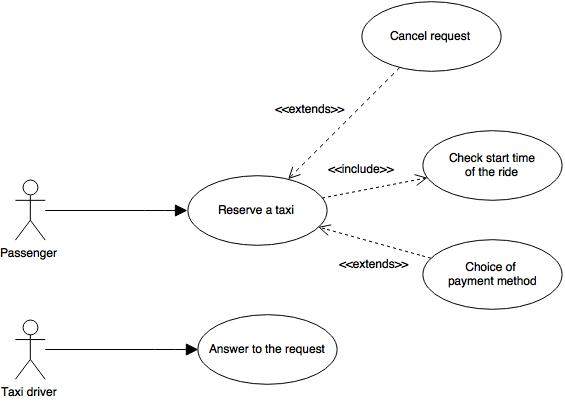
\includegraphics[scale=0.6]{Diagrams/UseCaseReserve.jpg}
					\end{figure}
				\end{center}
				
				\newpage
				
				\begin{figure}[h]
					\centering
					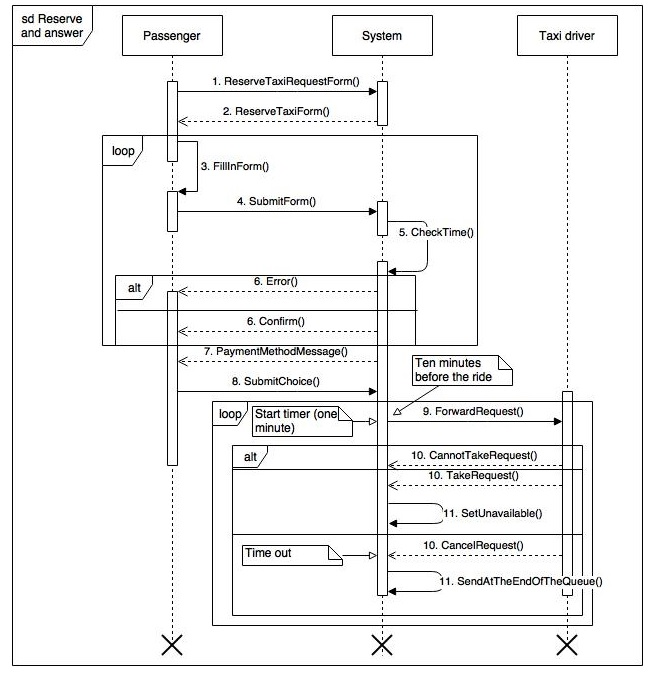
\includegraphics[scale=0.8]{Diagrams/SequenceReserve.jpg}
				\end{figure}
				\newpage
				\item Taxi Area
				\\ \\ \\
				\begin{center}
					\centering
					\begin{tabular}{|c|p{8cm}|}
						\hline \textbf{Actor} & Taxi driver.\\
						\hline \textbf{Goal} & See the taxi driver area.\\
						\hline \textbf{Input Condition} & The taxi driver is already logged in.\\
						\hline \textbf{Event Flow} & The taxi driver requests his area page.\\
						\hline \textbf{Output Condition} & The system shows the area page to the taxi driver.\\
						\hline \textbf{Exception} & If the information in the area is incorrect, the system refreshes the page.\\
						\hline
					\end{tabular}
					\vspace{4cm}
					\begin{figure}[h]
						\centering
						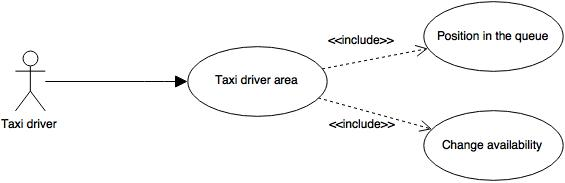
\includegraphics[scale=0.7]{Diagrams/UseCaseTaxiArea.jpg}
					\end{figure}
				\end{center}
			
				\newpage
				
				\begin{figure}[h]
					\centering
					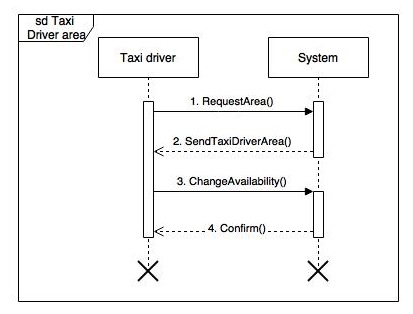
\includegraphics[scale=1]{Diagrams/SequenceTaxiArea.jpg}
				\end{figure}
	\end{itemize}
\newpage
	\subsection{State Chart diagram}
		This State Chart diagram describes the behaviour of the system.
		\\ \\ \\ \\ 
		\begin{figure}[h]
			\centering
			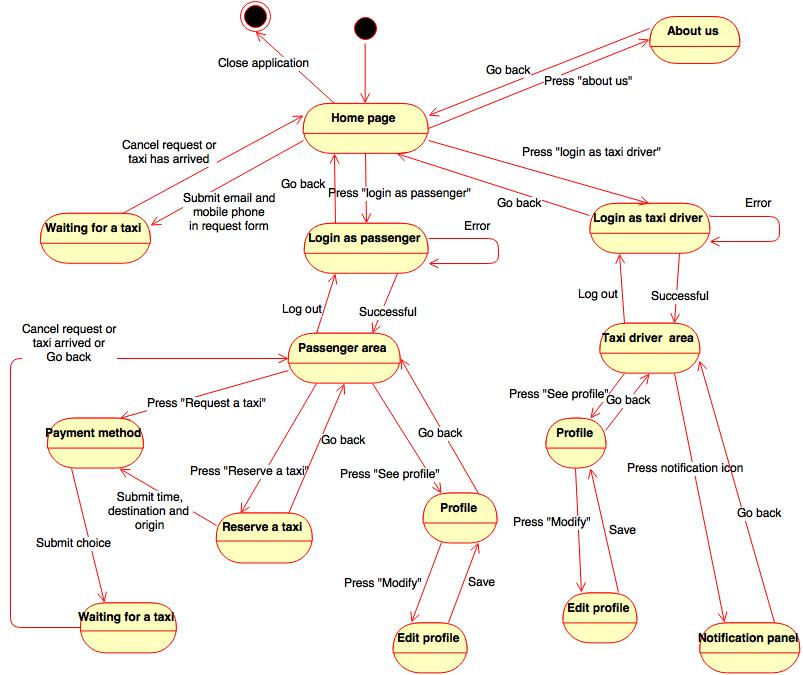
\includegraphics[scale=0.5]{Diagrams/stateChartDiagram.jpg}
		\end{figure}

\newpage
\section{Alloy Modeling}
	The alloy modeling has been used to test the consistency of the proposed Class diagram with the Alloy Analyzer 4.2. This report consists in the signatures of the classes, facts and assertions on the model and two examples of the world generated by our predicates.
	\subsection{Signatures}
	\begin{figure}[h]
		\centering
		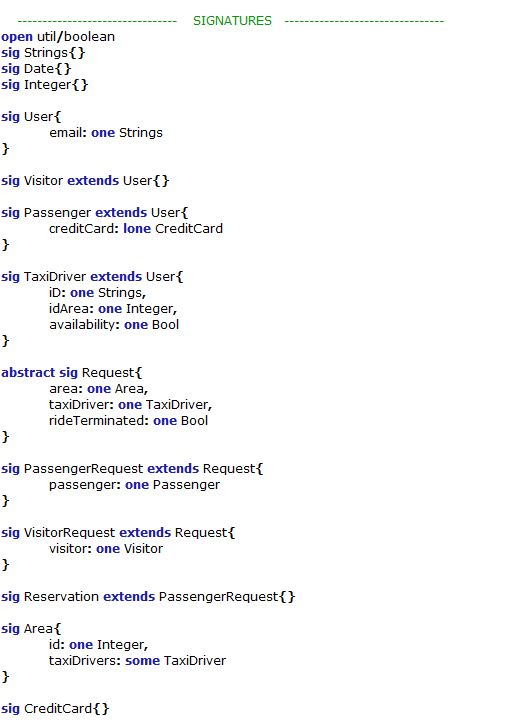
\includegraphics[scale=0.8]{Alloy/signatures.jpg}
	\end{figure}
\newpage
	\subsection{Facts}
	\begin{figure}[h]
		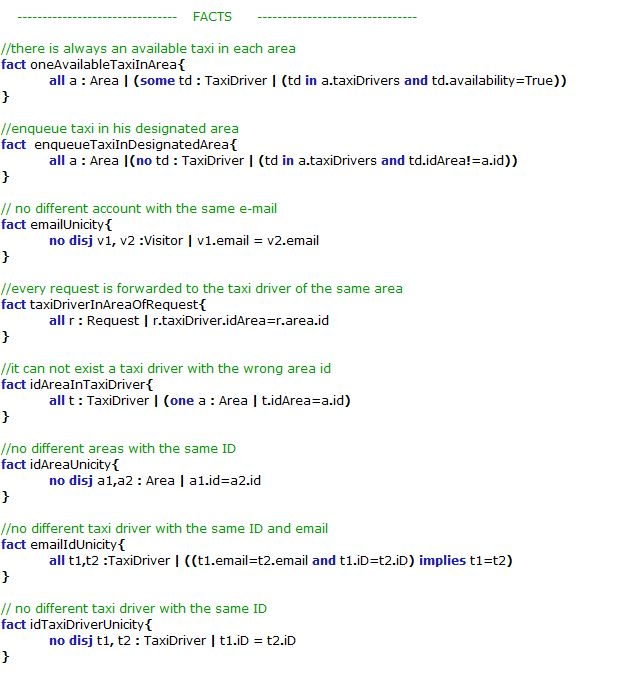
\includegraphics[scale=0.56]{Alloy/facts1.jpg}%
		\qquad\qquad
		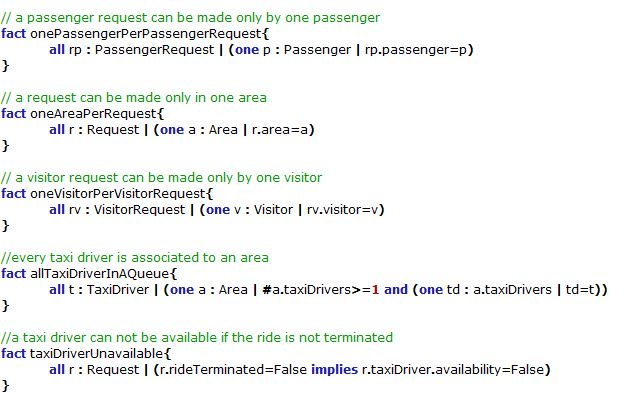
\includegraphics[scale=0.56]{Alloy/facts2.jpg}
	\end{figure}
\newpage
	\subsection{Assertions}
	\begin{figure}[h]
		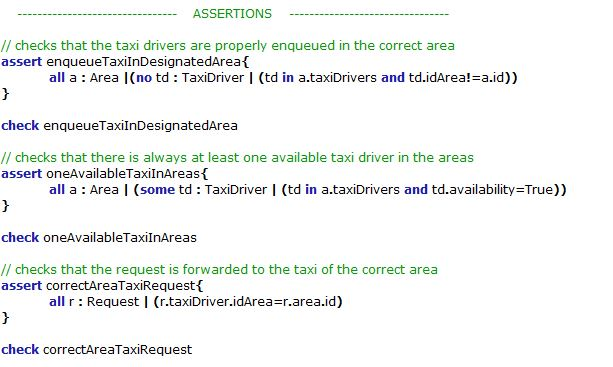
\includegraphics[scale=0.8]{Alloy/assertions.jpg}
	\end{figure}
	
	\subsection{Predicates}
		\begin{figure}[h]
			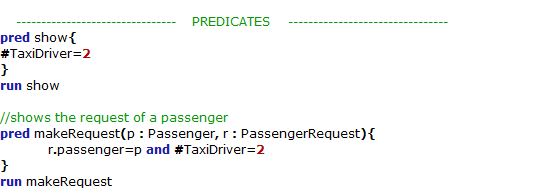
\includegraphics[scale=0.8]{Alloy/predicates.jpg}
		\end{figure}
\newpage
	\subsection{Results}
		\begin{figure}[h]
			\includegraphics[scale=1]{Alloy/results.jpg}
		\end{figure}
\newpage
	\subsection{Generated world}
		\subsubsection{General World}
		In this image is shown the world generated by Alloy Analyzer via the
		execution of the predicate "show".
		\\ \\ \\ \\ \\ \\
			\begin{figure}[h]
				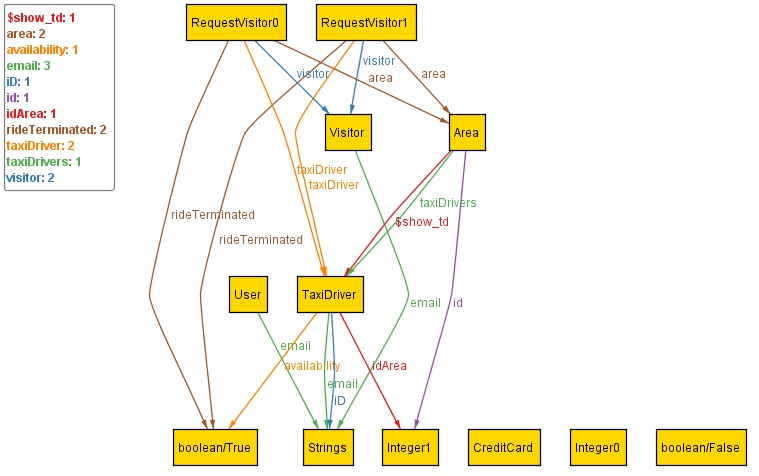
\includegraphics[scale=0.7]{Alloy/show.jpg}
			\end{figure}
\newpage
		\subsubsection{Request By A Passenger}
		In this image is shown the world generated by Alloy Analyzer via the
		execution of the predicate "makeRequest".
		\\ \\ \\ \\ \\ \\
		\begin{figure}[h]
			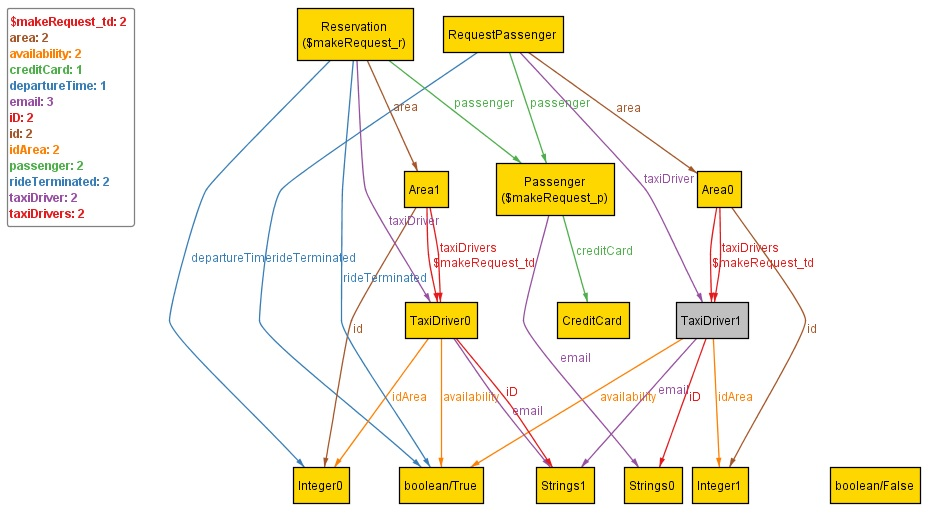
\includegraphics[scale=0.6]{Alloy/makeRequest.jpg}
		\end{figure}
\newpage
\section{Appendix}
	\subsection{Glossary}
		In order to avoid ambiguity, some words, which are often used in this document, are given a precise definition of what is the meaning in the contest of this project.
		\begin{itemize}
			\item User: a person who requests a service from the system. It can be a visitor or a passenger.
			\item Visitor: a person who is not registered in the application.
			\item Passenger: a person who is registered in the application.
			\item Taxi driver: a taxi driver who access the application with a specific ID.
			\item Request: the request of a taxi in a certain area and position in the city made by a user.
			\item Reservation: the reservation of a taxi in a certain area, place and time that can be made only by passengers.
	\end{itemize}
	\subsection{Software and tool used}
		\begin{itemize}
			\item TeXstudio (\url{http://www.texstudio.org/}): to redact and to format this document.
			\item draw.io (\url{https://www.draw.io/}):to create Use Case Diagrams, Sequence Diagrams, Class Diagrams and Statechart Diagrams.
			\item Balsamiq Mockups (\url{http://balsamiq.com/products/mockups/}): to create mockups.
			\item Alloy Analyzer (\url{http://alloy.mit.edu/alloy/}): to create Alloy models.
		\end{itemize}
	
	\subsection{Hours of work}
		Time spent redacting this document:
		\begin{itemize}
			\item Cattaneo Michela Gaia: {\raise.17ex\hbox{$\scriptstyle\sim$}}35 hours of work.
			\item Barlocco Mattia: {\raise.17ex\hbox{$\scriptstyle\sim$}}35 hours of work.
		\end{itemize}


\end{document}
